\documentclass[a4paper]{article}

\usepackage[english]{babel}
\usepackage[utf8]{inputenc}
\usepackage{amsmath}
\usepackage{amsthm}
\usepackage{amssymb}
\usepackage{booktabs}
\usepackage{graphicx}
\graphicspath{ {images/} }
\usepackage{physics}
\usepackage{subcaption}
\usepackage{hyperref}
\usepackage[export]{adjustbox}
\usepackage[framemethod=tikz]{mdframed}
\usepackage[colorinlistoftodos]{todonotes}

\newmdenv[
%  topline=false,
%  bottomline=false,
%  skipabove=\topsep,
%  skipbelow=\topsep
]{siderules}

\hypersetup{
	colorlinks=true,
	linktoc=all,
	linkcolor=blue,
}

\numberwithin{equation}{subsection}
\theoremstyle{definition}
\newtheorem{definition}{Definition}[section]

\newtheorem{theorem}{Theorem}[section]
 
\theoremstyle{remark}
\newtheorem*{remark}{Remark}

\newenvironment{definitionSR}
{
\begin{siderules}
\begin{definition}
}
{
\end{definition}
\end{siderules}
}

\newenvironment{theoremSR}
{
\begin{siderules}
\begin{theorem}
}
{
\end{theorem}
\end{siderules}
}

\DeclareMathOperator{\sign}{sign}
\newcommand{\Reals}{\mathbb{R}}
\newcommand{\Complex}{\mathbb{C}}
\newcommand{\ReP}[1]{
	\mathrm{Re}\pqty{#1}
}
\newcommand{\ImP}[1]{
	\mathrm{Im}\pqty{#1}
}
\newcommand{\ve}[1]{
	\mathbf{#1}
}
\newcommand{\cvb}[1]{
	[\mathbf{#1}]
}
\newcommand{\inv}[1]{
	{#1}^{-1}
}
\newcommand{\pdvc}[3]{
	\left(\pdv{#1}{#2}\right)_{#3}
}
\newcommand*{\conjugate}[1]{\overline{#1}}
\newcommand*{\conj}[1]{{#1}^*}
%\newcommand{\ip}[2]{
%	\langle {#1} | {#2} \rangle
%}
%\newcommand{\norm}[1]{\left\lVert#1\right\rVert}
\title{Notes for Math 121A}

\author{Harrison Bachrach}

\date{Spring 2015}


\begin{document}
\maketitle

\begin{abstract}
Notes for Math 121A based on lectures given by Dr.\ Nikhil Srivastava in Spring 2015 at UC Berkeley in Berkeley, California.
The following notes assume basic knowledge of series, multivariable calculus and linear algebra; however, the first few sections are dedicated to
the brief review of those topics.

For those of you scientists and engineers who have taken up to linear algebra \& multivariable calculus \emph{but no further},
I entreat you to continue reading. After the review, Sections~\ref{ComplexAnalysis} and~\ref{HarmonicAnalysis}
(on Complex Analysis and Harmonic Analysis respectively) demonstrate the humbling power and beauty of higher-level mathematics. 
While the topics are perhaps not expressed here with the rigor that would satisfy a mathematician,
I hope that they can offer a stimulating preview of ``upper division'' mathematics.

Sections suffixed with an asterix, i.e.\ the ``*'' symbol, are generally ``optional'' in that they don't \emph{necessarily} 
have applicability to the physical sciences. However, they are often quite beautiful and/or significant within pure mathematics.
\end{abstract}

\tableofcontents
\section{Notation}
\subsection{Screen \& Print Notation}
Many symbols of set theory and boolean logic are useful beyond their original applications.
In this section, I will be explaining the meaming of those symbols which are used here which you may not have encountered previously.
\begin{itemize}
\item A \textit{set} of things is denoted by curly braces. E.g.\ The set of natural numbers $\mathbb{N} = \Bqty{0, 1, 2, 3, \ldots}$. \\
\item The symbol $\in$ means ``in'' or ``is an element of''. For example, the statement $2 \in \mathbb{N}$ is true, while $ -3 \in \mathbb{N}$ is not.
\item The symbol $\forall$ means ``for all''. For example, $\forall x \in \mathbb{N} ~ x > -1$ is a true statement. \\
\item The symbol $\Rightarrow$ means ``implies'', that is, ``$p \Rightarrow r$'' is to be read as ``if $p$ is true, then $q$ is also true''.
Note that it states nothing about the status of $p$ if we are given the status of $q$,
nor does it tell us the status of $q$ if $p$ is false. \\
\item The symbol $\iff$ means ``if and only if''\footnote{``if and only if'' is often written as ``iff''}, that is, ``$p \iff r$'' is to be read as ``if and only if $p$ is true, then $q$ is also true'' \emph{and} ``if and only if $q$ is true, then $p$ is also true.'' Intuitively, this logically links $p$ and $q$.
\item The symbol $\wedge$ means ``and''. A statement ``$P(x) \wedge Q(x)$'' is only true if \emph{both} $P(x)$ and $Q(x)$ are true statements. 
E.g., $(5>3 \wedge 2 \neq 0)$ is true, while $(3>6 \wedge 4 = 4)$ is false. \\
\item We can build sets by using \textit{set builder notation}.
The notation works as follows: a set $S$ of elements that satisfy a condition is denoted 
\[
	S = \Bqty{\text{Element}~|~\text{Condition on element}}.
\]
For example, the set of natural numbers can be expressed as 
\[
	\mathbb{N} = \Bqty{x~|~x \in \mathbb{Z} \wedge x \geq 0}
\]
where $\mathbb{Z}$ is the set of integers. \\
\item A very useful notation for talking about intervals on the real line is \textit{interval notation}. It works as follows:
\begin{align*}
(a,b) &= \Bqty{x~|~x \in \Reals \wedge a<x<b} \\
[a,b) &= \Bqty{x~|~x \in \Reals \wedge a\leq x<b} \\
(a,b] &= \Bqty{x~|~x \in \Reals \wedge a<x\leq b} \\
[a,b] &= \Bqty{x~|~x \in \Reals \wedge a\leq x\leq b} \\
\end{align*} \\


\end{itemize}
\subsection{Handwritten Notation}
%%%% SERIES

\section{Series}
\begin{definitionSR}
A \textit{series} is the sum of the items in a sequence.
\end{definitionSR}


\emph{Finite} sums are always well defined, while \emph{infinite} sums must meet certain criteria to be well defined. A finite sum up to term $a_N$ would be denoted
\[
	\sum_{n=0}^N a_n = S_N
\]
While an infinite sum, that is the limit of a finite sum (assuming the limit exists) is denoted as
\[
	\lim_{N \to \infty} S_N = \lim_{N \to \infty} \sum_{n=0}^N a_n = \sum_{n=0}^\infty a_n = S
\]
If the above limit exists, the series is \textit{convergent}, while if it doesn't, the series is \textit{divergent}.

\begin{definitionSR}
A \textit{geometric series} is one where terms are related by a common ratio $r$. The general geometric series up to order $N$ could be expressed as
  \[
      S_N = a + ar + ar^2 + \cdots + ar^N = S_N
  \]
The formula for a finite geometric series is
  \begin{equation}
  S_N = \frac{a(1-r^N)}{1-r}
  \end{equation}
and the formula for an infinite geometric series (assuming the series exists, i.e.\ assuming $|r|<1$) is simply (by taking the limit $N \to \infty$),
  \begin{equation}
  S = \frac{a}{1-r}
  \end{equation}
where in both cases, a and r represent the first term and common ratio, respectively.\\
\end{definitionSR}


\begin{definitionSR}
The \textit{remainder} $R_N$ is the difference between the infinite series $S$ and the ``partial sum'' $S_N$, that is,
\[
	R_N = \sum_{k=N+1}^\infty a_k = S-S_N
\]
\end{definitionSR}

Series are a way of breaking something difficult into a sum of easy to handle terms.

\subsection{Tests for Convergence}

\begin{definitionSR}[Comparing Magnitudes]
\[
 f \ll g \iff \lim_{n \to \infty } \frac{f(n)}{g(n)} = 0
\]
\end{definitionSR}

Do note some general relative magnitudes of growth:
\begin{equation}
\log n \ll n \ll n^2 \ll \ldots \ll 2^n \ll n!
\end{equation}

\subsubsection{Preliminary Test}
If $\lim_{n \to \infty} a_n \neq 0$, then $\sum_n^\infty a_n$ diverges.

\subsubsection{Integral Test}
If $a_n$ is non-negative and non-increasing, then
\[
	\sum_{n=1}^\infty a_n \text{\, converging} \iff \int_b^\infty a(x)\,dx \text{\, converging}
\]
where $a(x)$ is the continuation of $a_n$ for the real variable $x$; e.g.\ if $a_n = 1/n$, then $a(x) = 1/x$, where $x \in \mathbb{R}$.
\subsubsection{Comparison Principle}
Suppose $a_n$ and $b_n$ are sequences with $0 \leq a_n \leq b_n$ for all $n$.
\begin{align*}
\sum b_n \text{\, converges}  &\Rightarrow \sum a_n \text{\, converges.} \\
\sum a_n \text{\, diverges}  &\Rightarrow \sum b_n \text{\, diverges.}
\end{align*}

\subsubsection{Special Comparison Principle}
If $a_n$, $b_n$ are non-negative sequences and $\lim_{n \to \infty} \frac{a_n}{b_n} < \infty$ (that is to say, the limit is finite), then
\[
\sum b_n \text{\, converges}  \Rightarrow \sum a_n \text{\, converges.} 
\]

\subsubsection{Ratio Test}
Defining
\begin{center}
\begin{tabular}{cc}
$ \rho_n = \displaystyle \left|\frac{a_{n+1}}{a_n}\right| $, & $ \rho = \displaystyle \lim_{n \to \infty} \rho_n = \displaystyle \lim_{n \to \infty} \displaystyle \left|\frac{a_{n+1}}{a_n}\right| $
\end{tabular}
\end{center}
then
\begin{align*}
\rho < 1 &\Rightarrow \text{the series converges.} \\
\rho > 1 &\Rightarrow \text{the series diverges.} \\ 
\rho = 1 &\Rightarrow \text{the test is inconclusive.}
\end{align*}

\subsubsection{Alternating Series Test}
If $a_n$ is an alternating series (i.e., $\sign(a_{n+1}) = -\sign(a_n)$), $|a_{n+1}| \leq |a_n|$, \emph{and} $\lim_{n \to \infty} = 0$, then the series converges.
	
Note: if $\sum |a_n|$ converges, the series is \textit{absolutely convergent}.

\subsection{Power Series}
\begin{definitionSR}
A \textit{power series} is a function expressed as an infinite sum of monomials. That is, a function $f(x)$ can be expanded in a power series if it can be expressed as
\[
f(x) = \sum_{n=0}^\infty a_n x^n
\]
for some $\{a_n\}$.
\end{definitionSR}

\begin{theoremSR}
A power series expansion of $f(x)$ converges on only 3 types of intervals.
\begin{enumerate}
\item It converges everywhere (that is, $\forall x$)
\item It converges for $x=0$ only
\item It converges when $|x|<R$ and diverges when $|x|>R$, where $R$ is the radius of convergence. (The points $x=\pm R$ must be checked explicitly and are not, in general, symmetric.)
\end{enumerate}
\end{theoremSR}

\subsubsection{Taylor Series}

\begin{definitionSR}
The power series expansion of an analytic function about a number $a$ is known as a \textit{Taylor series}. When $a=0$, this is known as a \textit{Maclaurin series}. If $f(x)$ is analytic,
\[
f(x-a) = f(a) + f'(a)(x-a) + \frac{f''(a)}{2!}(x-a)^2 + \cdots + \frac{f^{(n)}}{n!}(x-a)^n + \cdots
\]
Note: the radius of convergence for Taylor series depends upon $a$.
\end{definitionSR}

Here are some common Maclaurin series, with their interval of convergence in parentheses:\\
\newline

\begin{adjustbox}{center}
\begin{tabular}{rclr}

$\sin(x) \quad = $&$  \displaystyle \sum_{n=0}^\infty \frac{(-1)^n x^{2n+1}}{(2n+1)!} $&$ = \quad \displaystyle x - \frac{x^3}{3!} + \frac{x^5}{5!} - \frac{x^7}{7!} + \cdots$ & $ (x \in \Reals) $\\

\midrule

$\cos(x) \quad = $&$   \displaystyle  \sum_{n=0}^\infty \frac{(-1)^n x^{2n}}{(2n)!} $&$ = \quad \displaystyle 1 - \frac{x^2}{2!} + \frac{x^4}{4!} - \frac{x^6}{6!} + \cdots$ & $ (x \in \Reals) $\\


\midrule

$e^x \quad = $&$ \displaystyle \quad \sum_{n=0}^\infty \frac{x^n}{n!} $&$ = \quad \displaystyle 1 + x + \frac{x^2}{2!} + \frac{x^3}{3!} + \cdots$ & $ (x \in \Reals) $\\

\midrule

$\log(1+x) \quad =  $&$  \displaystyle \quad \sum_{n=1}^\infty \frac{(-1)^{n+1}x^n}{n} $&$ = \quad \displaystyle x - \frac{x^2}{2} + \frac{x^3}{3} - \frac{x^4}{4} \cdots$ & $ (x \in (-1,1]\,) $\\

\midrule

$(1+x)^p \quad = $&$ \displaystyle \quad \sum_{n=0}^\infty \binom{p}{n} x^n $&$ = \quad \displaystyle 1 + px + \frac{p(p-1)}{2!}x^2  + \frac{p(p-1)(p-2)}{3!}x^3 + \cdots$ & $ (x \in (-1,1)\,) $\\

\end{tabular}
\end{adjustbox}

\subsubsection{Asymptotic Notation}
How do we write higher order terms we are not concerned with so that we can keep track of them? With ``Little-oh'' and ``Big-Oh'' notation!

\begin{definitionSR}[Little-oh notation]
Given continuous functions $f(x)$ and $g(x)$, we say that $f(x) = o(g(x))$ as $x \to a$ if
\[
\lim_{x \to a} \frac{f(x)}{g(x)} = 0
\]
e.g.\ $x^5 = o(x)$ as $x \to 0$, $x^4 = o(x^5)$ as $x \to \infty$, etc.
\end{definitionSR}

\begin{definitionSR}[Big-Oh notation]
Given continuous functions $f(x)$ and $g(x)$, we say that $f(x) = (g(x))$ as $x \to a$ if
\[
\lim_{x \to a} \left|\frac{f(x)}{g(x)}\right| < \infty
\]
e.g.\ $x^2 = O(x^2)$ as $x \to 0$, $2\sin x = O(1)$ as $x \to \infty$, etc.
\end{definitionSR}

The rules for manipulating the notation is as follows:

\begin{enumerate}
\item If $c \in \Reals$ and $f(x) = o(g(x))$, then $cf(x)=o(g(x))$.

\item If $f_1(x) = o(g_1(x))$ and $f_2(x) = o(g_2(x))$, then $f_1(x)f_2(x) = o(g_1(x)g_2(x))$.

\item If $f(x) = o(g(x))$, then $x\cdot f(x) = o(x\cdot g(x))$.

\item If $\displaystyle \lim_{x \to 0} g(x) = 0$, then $\displaystyle \frac{1}{1+g(x)} = 1 - g(x) + o(g(x))$.

\item $o(f(x)+g(x)) = o(f(x)) + o(g(x))$

\item $o(o(f(x))) = o(f(x))$

\end{enumerate}

All of the above apply to ``Big-Oh'' notation as well.

Both notations are commonly used in expressing series so that one can keep track of the order of an approximation. For example, if we expand $e^x$ about $x=0$ but are only concerned with second-order terms and below, we can write it as 
\[
e^x = 1+x+\frac{x^2}{2!}+o(x^2) = 1+x+\frac{x^2}{2!} + O(x^3)
\]

\subsection{Error of Series Approximations}
In general, the error for a finite \emph{power} series can be expressed as 
\begin{align}
R_N(x) &= f(x) - \left( f(x) + (x-a)f'(a) + \cdots + (x-a)^N \frac{f^{(N)}(a)}{N!}\right) \\
&= \frac{(x-a)^{N+1}f^{(N+1)}(c)}{(N+1)!}
\end{align}

for some $c \in [a,x]$. This is known as \textit{Taylor's Theorem}. However, it is not of much practical use, as we do not have a formula for $c$.

In the case where the power series coefficients are \emph{decreasing} and \emph{non-negative}, on the interval $x \in (-1,1)$ we can use the formula
\begin{equation}
R_N(x) = \frac{a_{N+1}x^N}{1-|x|}
\end{equation}

In the case where the (not necessarily power) series is \emph{alternating}, and absolutely decreasing (that is, $|a_{n+1}|<|a_n|$ for all $n$) and $\lim_{n \to \infty} a_n = 0$, then 
\begin{equation}
|R_N| \leq |a_{N+1}|.
\end{equation}


%%%%% LINEAR ALGEBRA

\section{Linear Algebra}

\subsection{Notation}

\begin{itemize}
\item A \textit{vector} in a vector space is denoted as $\ve{x}$.
\item The \textit{coordinate vector} of $\ve{x}$ with respect to a basis $\mathcal{B}$ is denoted as $\cvb{x}_\mathcal{B}$. If there is no subscript, e.g.\ $\cvb{x}$, the basis is understood to be the \textit{standard basis}.
\item The \textit{standard basis elements} are denoted $\ve{e}_1, \ve{e}_2, \ldots \ve{e}_n$.
\end{itemize}

\subsection{Inner Product Spaces}

\begin{definitionSR}
An \textit{inner product} is a billinear map that takes two vectors of a vector space and returns a scalar of a field $F$ (in almost all cases, $F=\Reals$ or $F=\Complex$).
In more symbolic notation, we have $\langle \cdot , \cdot \rangle : V \times V \to F$. A billinear map qualifies as an inner product if all of the following conditions are
met\footnote{Where $z^*$ is the complex conjugate of $z$, also written as $\bar{z}$. For more information, see Section~\ref{ComplexNumbers}.}:
\begin{enumerate}
\item $\braket{\ve{x}}{\ve{x}} \geq 0$ and $\braket{\ve{x}}{\ve{x}} = 0 \iff \ve{x} = \ve{0}$
\item $\braket{a_1\ve{x}_1 + a_2\ve{x}_2}{\ve{y}} = a_1^*\braket{\ve{x}_1}{\ve{y}} + a_2^*\braket{\ve{x}_2}{\ve{y}}$
\item $\braket{\ve{x}}{b_1\ve{y}_1 + b_2\ve{y}_2} = b_1\braket{\ve{x}}{\ve{y}_1} + b_2\braket{\ve{x}}{\ve{y}_2}$
\item $\braket{\ve{x}}{\ve{y}} = \braket{\ve{y}}{\ve{x}}^*$
\end{enumerate}

\end{definitionSR}
\begin{definitionSR}
The \textit{norm} of a vector $\ve{x}$ is $\norm{\ve{x}} = \sqrt{\braket{\ve{x}}{\ve{x}}}$.
\end{definitionSR}

From these we get a few theorems, which we will state here without proof.

First we have the \textit{Cauchy-Schwarz Inequality}:
\begin{equation}
\braket{\ve{p}}{\ve{q}} \leq \norm{\ve{p}}\cdot\norm{\ve{q}}.
\end{equation}
Next we have the \textit{Triangle Inequality}:
\begin{equation}
\norm{\ve{p} + \ve{q}} \leq \norm{\ve{p}} + \norm{\ve{q}}.
\end{equation}
Lastly we have the \textit{Pythagorean theorem}:
\begin{equation}
\braket{\ve{p}}{\ve{q}} = 0 \iff \norm{\ve{p}}^2 + \norm{\ve{q}}^2 = \norm{\ve{p} + \ve{q}}^2.
\end{equation}

For our purposes, there are only four important inner products to concern ourselves with. When we're dealing with vectors in $\Reals^n$, we will use the familiar \textit{dot product}; if $\vb{x}, \vb{y} \in \Reals^n$, then 
\begin{equation}
\braket{\vb{x}}{\vb{y}} = \vb{x}^T \vb{y} = \sum_{i=1}^n x_i y_i
\end{equation}
With vectors  $\vb{x}, \vb{y} \in \Complex^n$ we have a similarly defined inner product defined thusly:
\begin{equation}
\braket{\vb{x}}{\vb{y}} = \vb{x}^\dagger \vb{y} = \sum_{i=1}^n x_i^* y_i
\end{equation}

For functions/vectors in $L^2(X)$ meaning\footnote{where $X$ is most commonly $[a,b]$ or $\Reals$} the set of functions $\{f_i\}$ that satisfy 
\[
\int_X |f_i(x)|^2\, dx < \infty 
\]

\subsection{Coordinates and Change of Bases}

The coordinate mapping of a transformed vector $T(\ve{x})$ is given simply as

\begin{equation}
[T(\ve{x})] = 
\begin{bmatrix}
[T(\ve{e}_1)]&[T(\ve{e}_2)]&\cdots&[T(\ve{e}_n)]\\
\end{bmatrix}
\cvb{x} = [T]\cvb{x}.
\end{equation}

In a basis $\mathcal{B}$ with basis $\{\ve{b}_i\}$, the transformation can be written

\begin{equation}
[T(\ve{x})]_\mathcal{B} = 
\begin{bmatrix}
[T(\ve{b}_1)]_\mathcal{B}&[T(\ve{b}_2)]_\mathcal{B}&\cdots&[T(\ve{b}_n)]_\mathcal{B}\\
\end{bmatrix}
\cvb{x}_\mathcal{B} = [T]_\mathcal{B}\cvb{x}_\mathcal{B}.
\end{equation}

To switch between these two transformation matrices, we have
\begin{equation}
[T]=B[T]_\mathcal{B}\inv{B} \iff [T]_\mathcal{B} = \inv{B}[T]B
\end{equation}

where

\begin{equation}
B = \begin{bmatrix} 
[\ve{b}_1]&[\ve{b}_2]& \cdots & [\ve{b}_n]\\

\end{bmatrix}.
\end{equation}

From the above, we can see
\begin{equation}
\cvb{x} = B\cvb{x}_\mathcal{B} \iff \cvb{x}_\mathcal{B} = \inv{B}\cvb{x}.
\end{equation}

\subsection{Diagonalization}
\begin{definitionSR}
To \textit{diagonalize} a matrix $A$ is to express it as $A=CD\inv{C}$, where $C$ is an invertible matrix and $D$ is a diagonal matrix.
\end{definitionSR}
TODO: How to diagonalize a matrix.

\begin{definitionSR}
An \textit{orthogonal matrix} is a real matrix which has the following (mutually equivalent) properties:
\begin{enumerate}
\item All its columns (if treated as column vectors) are mutually orthogonal.
\item Its transpose equals its inverse, e.g.\ if $Q$ is an orthogonal matrix, $Q^T = \inv{Q}$.
\end{enumerate}

\end{definitionSR}

\begin{theoremSR}
	If $A$ is \textit{symmetric} (i.e.\ $A = A^T$), then it also has the following properties:
	\begin{enumerate}
	\item It is diagonalizable as $A=QDQ^T$, where $D$ is a diagonal matrix and $Q$ is a orthogonal matrix.
	\item Its basis is orthogonal.
	\item All its eigenvalues are real.
	\end{enumerate}
\end{theoremSR}

\begin{definitionSR}
The \textit{adjoint} of a matrix $A$ is $A^\dagger = (A^T)^*$. This is pronounced ``A dagger.'' 
In physics, 
this is commonly known as the \textit{Hermitian conjugate} of $A$.
\end{definitionSR}
\begin{definitionSR}
An \textit{unitary matrix} is a complex matrix which has the following (mutually equivalent) properties:
\begin{enumerate}
\item All its columns (if treated as column vectors) are mutually orthogonal.
\item Its adjoint equals its inverse, e.g.\ if $Q$ is a unitary matrix, $Q^\dagger = \inv{Q}$.
\end{enumerate}
\end{definitionSR}


\begin{theoremSR}
	If $A$ is \textit{Hermitian} (i.e.\ $A = A^\dagger$), then it also has the following properties:
	\begin{enumerate}
	\item It is diagonalizable as $A=UDU^\dagger$, where $D$ is a diagonal matrix and $U$ is a unitary matrix.
	\item Its basis is orthogonal.
	\item All its eigenvalues are real.
	\end{enumerate}
\end{theoremSR}

\section{Partial Differentiation}
\begin{definitionSR}
A \textit{partial derivative} is the multivariate analogue of a traditional derivative.
\[
\pdv{f}{x_i} = \lim_{\Delta x_i \to 0} \frac{f(x_1,\cdots, x_i + \Delta x_i, \cdots, x_n) - f(x_1,\cdots, x_i, \cdots, x_n)}{\Delta x_i}
\]
\end{definitionSR}

What this means in a practical context is that when taking a partial derivative, we take all other variables to be constant.
E.g.\ $f(x,y) = 3x^2\cos(y)$ 
\[
\pdv{f}{x} = 6x\cos(y), \quad  \pdv{f}{y} = -3x^2 \sin(y)
\]

A function is \textit{differentiable} at a point if it is well approximated by a linear function in the neighborhood of that point.

Let's say we have a function $z = f(x,y)$. We can then approximate small changes in $z$ like so:
\[
\Delta z = f(x_0 + \Delta x, y_0 + \Delta y) - f(x_0,y_0) = \pdv{f}{x} \Delta x + \pdv{f}{y} \Delta y + o(\Delta x) + o(\Delta y)
\]

Taking the limit of the above, we get the total differential
\begin{equation}
dz = \pdv{f}{x} dx + \pdv{f}{y} dy
\end{equation}

If we have more than 2 variables of concern in a problem, e.g.\ $z = f(x,y)$ and $z = g(x, \theta)$, 
then we can use a subscript to denote what variable(s) we are holding constant,
\[
\pdvc{z}{x}{\theta} = \pdv{g}{x}, \quad \pdvc{z}{x}{y} = \pdv{f}{x}
\]

\subsection{Implicit Partial Differentiation}
Careful manipulation of total differentials can yield partial derivatives for complicated equations. For example, given $x^2 + y^2 + z^2 = 1$, what is $\pdvc{z}{x}{y}$?
We can manipulate differentials as if they were algebraic quantities to generate this derivative, 
but we must understand that ``under the hood,'' 
we are really manipulating these ``$\Delta x$'' type quantities (which are \emph{not} symbolic in the same manner as differentials)
and then subsequently taking the \emph{limit} as described in the definition of the partial derivative.

If we consider this equation $x^2 + y^2 + z^2 = 1$ a constant function, that is, $F(x,y,z)=x^2 + y^2 + z^2 = 1$, then
\[
dF = 2x\,dx + 2y\,dy + 2z\,dz
\]
Now, we are holding $y$ constant, so $\Delta y = 0$, thus we are interested in
\[
dF_y = 2x\,dx + 2z\,dz
\]
where the subscript $y$ denotes that we are taking $y$ as constant. Since $F$ is a constant function, its differential must be zero. Thus,
\begin{align*}
2x\,dx + 2z\,dz &= 0 \\
2x\,dx &= -2z\,dz\\
\pdvc{z}{x}{y} &= -\frac{x}{z} \\
\end{align*}

\subsection{The Chain Rule}
\begin{figure}[h]
	\caption{The chain rule, visualized}
	\begin{subfigure}[h]{0.3\textwidth}
	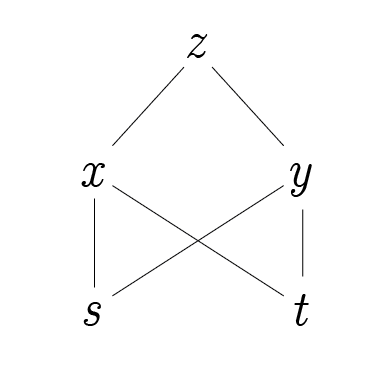
\includegraphics[width=\textwidth]{chain_rule_diagram-01}
	\caption{Interdependancies of variables in example}
	\end{subfigure}
	~~
	\begin{subfigure}[h]{0.3\textwidth}
	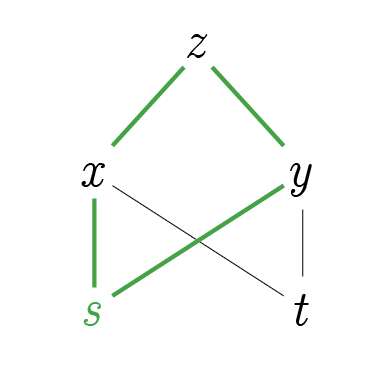
\includegraphics[width=\textwidth]{chain_rule_diagram-02}
	\caption{``Connections'' used when finding $\pdvc{z}{s}{t}$}
	\label{fig:chain2}
	\end{subfigure}
	~~
	\begin{subfigure}[h]{0.3\textwidth}
	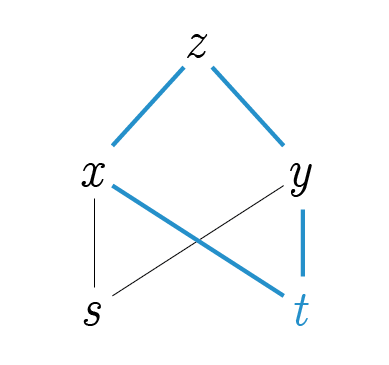
\includegraphics[width=\textwidth]{chain_rule_diagram-03}
	\caption{``Connections'' used when finding $\pdvc{z}{t}{s}$}
	\end{subfigure}
\end{figure}

Just as in single variable calculus, when we differentiate compositions of two or more functions, we have to use the chain rule.
However, the process is slightly more complicated than in the single-variable case. 
Again, we are going to utilize the \textit{total differential}.
While we \emph{can} use a formula like we do in the single-variable case,
it is fairly cumbersome, difficult to remember, and not as illuminating as the alternative.

Suppose we have $z = z(x,y)$, $x = x(s,t)$, and $y=y(s,t)$. 
We know from earlier that
\begin{align}
dz &= \pdv{z}{x} dx + \pdv{z}{y} dy \\
dx &= \pdv{x}{s} ds + \pdv{x}{t} dt \\
dy &= \pdv{y}{s} ds + \pdv{y}{t} dt 
\end{align}
Now, suppose we are interested in $\pdvc{z}{s}{t}$.
In this case, we are holding $t$ constant, and as a result, we may remove any term with $dt$.
Thus,

\begin{align}
dz &= \pdv{z}{x} dx + \pdv{z}{y} dy \\
dx &= \pdv{x}{s} ds  \\
dy &= \pdv{y}{s} ds  
\end{align}

Recalling that, in truth, we are manipulating these ``$\Delta x$'' type quantites,
we may use the principle of substitution. Thus,
\begin{equation}
dz_t = \pdv{z}{x} \pdv{x}{s} ds + \pdv{z}{y} \pdv{y}{s} ds = \pqty{\pdv{z}{x} \pdv{x}{s} + \pdv{z}{y} \pdv{y}{s} } ds
\end{equation}
If we bring the $ds$ to the other side (by utilizing the fact we are manipulating ``$\Delta x$'' type quantities), we get
\begin{equation}
\pdvc{z}{s}{t}=  \pdv{z}{x} \pdv{x}{s} + \pdv{z}{y} \pdv{y}{s}
\end{equation}
As you can see, the chain rule can be understood as the ``chains'' of dependence between variables.
If you look at Figure~\ref{fig:chain2} on page~\pageref{fig:chain2}, you can see the tree-like structure of the system of variables. 
Each term represents a pathway down from the function of interest to the independent variable that is not fixed.
Each line connecting two variables represents a derivative of the higher w.r.t.\ the lower.

\subsection{Optimization}
\subsubsection{Gradient}
\subsubsection{Lagrange Multipliers}

%%%%%%%%%% COMPLEX ANALYSIS %%%%%%%%%%%
\section{Complex Analysis}
\label{ComplexAnalysis}
\subsection{Complex Numbers}
\label{ComplexNumbers}
\begin{definitionSR}
The \emph{imaginary unit}, denoted as $i$, is the solution to the following equation:
\[
i^2 = -1
\]
\end{definitionSR}
From this, we can generate a definition of the Complex Numbers.
\begin{definitionSR}
The \emph{set of complex numbers}, denoted $\Complex$, can be defined as
\[
\Complex = \Bqty{x+iy ~ | ~ x,y \in \Reals}
\]
\end{definitionSR}
We also define the functions $\ReP{x+iy}=x$ and $\ImP{x+iy}=y$ to work with the real and imaginary parts more easily.
Two complex numbers are equal if and only if their corresponding real and imaginary parts are both equal. That is,
\[
z_1 = z_2 \iff \ReP{z_1} = \ReP{z_2} \wedge \ImP{z_1} = \ImP{z_2}.
\]
\begin{figure}[h]
	\centering
	\caption{The complex conjugate of $z$, visualized}
	\label{fig:complexAddition}
	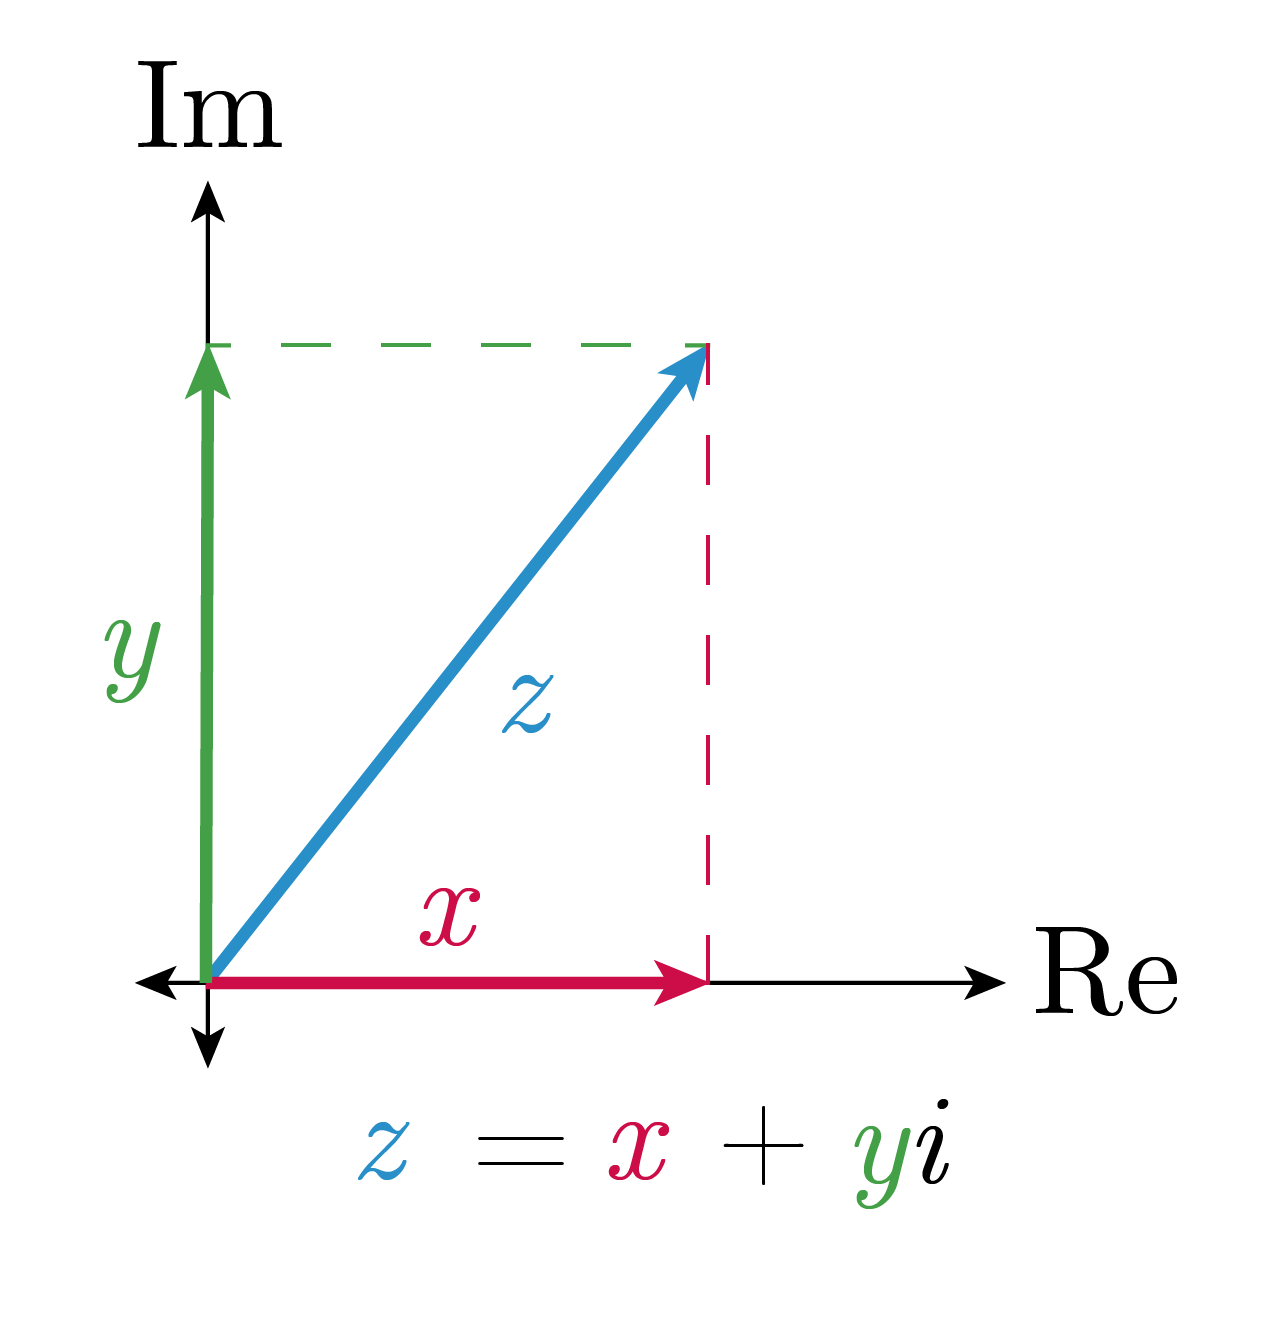
\includegraphics[width=3in]{complex_number_diagram-01}
\end{figure}
We can think of complex numbers as analogous to Euclidean vectors with
the real and imaginary lines as the $x$ and $y$ axes. See Figure~\ref{fig:complexAddition}. 
Addition and subtraction are defined relatively simply enough:
\[
z_1 \pm z_2 = (x_1 + i y_1) \pm (x_2 + i y_2) = (x_1 \pm x_2) + i (y_1 \pm y_2)
\]
Multiplication follows what you'd expect:

\begin{align*}
z_1 \cdot z_2 &= (x_1 + i y_1)(x_2+ i y_2)\\
&= x_1 x_2 + i x_2 y_1 + i x_1 y_2 + i^2 y_1 y_2\\
&= (x_1 x_2 - y_1 y_2) + i(x_2 y_1 + x_1 y_2)
\end{align*}

For division, what we are really asking is, 
``given that $z \neq 0$, does $\inv{z}$ exist $\forall z$ such that $z \inv{z} = 1$, and if so, what is it?'' 
Reformulating the question we get,
``given $z = x + iy \neq 0$, what is $\inv{z} = a + ib$ such that $(x+iy)(a+ib) = 1$?''
Expanding this out gives us
\[
(xa - yb) + i(ya + xb) = 1 + 0i
\]
From the definition of equality for complex numbers that we saw earlier,
the real and imaginary parts of two complex numbers must be equal if the the complex numbers are to be equal. Thus,
\begin{align*}
xa - yb &= 1 \\
ya + xb &= 0
\end{align*}
Noting that this is simply a system of linear equations, we can put it into matrix form,
\[
\pmqty{x & -y \\ y & x} \pmqty{a \\ b} = \pmqty{1 \\ 0}
\]
Since 
\[
\det \pmqty{x & -y \\ y & x}  = x^2 + y^2 \neq 0
\]
the matrix is invertable, thus $a$ and $b$ exist and are unique, given by
\begin{align*}
\pmqty{a \\ b} &= \inv{\pmqty{x & -y \\ y & x}} \pmqty{1 \\ 0} \\
&= \frac{1}{x^2 + y^2} \pmqty{x & y \\ -y & x } \pmqty{1 \\ 0} \\
&= \pmqty{\frac{x}{x^2+y^2} \\ \frac{-y}{x^2+y^2}} \\
\end{align*}

Thus, if $z \neq 0$, then
\[
\inv{z} = \frac{x}{x^2+y^2} + i \frac{-y}{x^2+y^2}
\]
\begin{definitionSR}
The \textit{complex conjugate} of a complex number $z$
(or often times, simply the \textit{conjugate} of $z$),
denoted\footnote{Physicists tend to use the $\conj{z}$ notation,
while mathematicians use the $\conjugate{z}$ notation.}
with either a star or overbar (e.g.\ $\conj{z}$ or $\conjugate{z}$),
is the negation of $z$'s imaginary part. That is, if $z = x+iy$, then
\[
\conj{z} = x-iy.
\]

\end{definitionSR}
Some important properties of the complex conjugate are as follows
(assuming $z_1, z_2 \in \Complex$):
\begin{itemize}
\item $\conjugate{z_1+z_2} = \conjugate{z_1} + \conjugate{z_2}$
\item $\conjugate{z_1 z_2} = \conjugate{z_1} \conjugate{z_2}$
\item $\conjugate{\inv{z_1}} = \inv{(\conjugate{z_1})}$

\begin{figure}[h]
	\centering
	\caption{The complex conjugate of $z$, visualized}
	\label{fig:conjugate}
	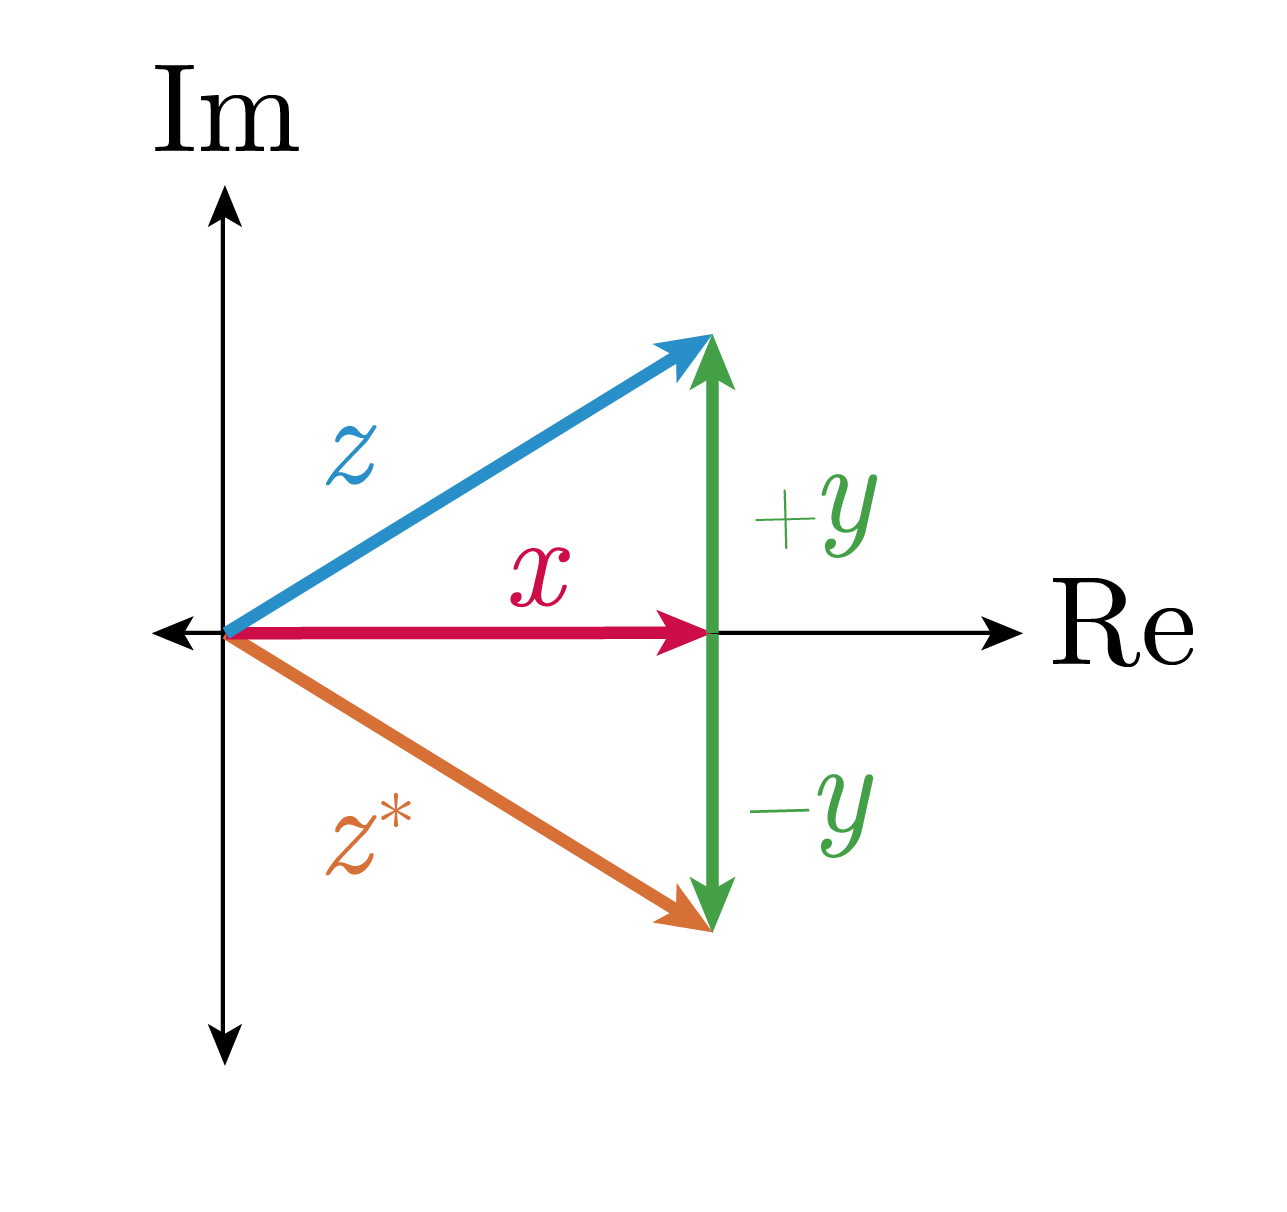
\includegraphics[width=3in]{complex_number_diagram-03}
\end{figure}
\end{itemize}
One can think of complex conjugation of a reflection a complex coordinate about the real axis;
see Figure~\ref{fig:conjugate}.

\begin{definitionSR}
The \textit{absolute value} or \textit{magnitude} of a 
complex number $z$, denoted $\abs{z}$, is the ``length'' of the Euclidean vector from the origin 
to the point $z$ in the $\Complex$ plane. If $z=x+iy$ where $x,y \in \Reals$,
\[
\abs{z} = \sqrt{x^2 + y^2}
\]
\end{definitionSR}

The absolute value of a complex number is a type of norm, specifically the
\textit{Euclidean norm} or the $L^2$ \textit{norm}. 
Some useful properties of the absolute value include:
\begin{itemize}
\item $\abs{z_1 z_2} = \abs{z_1} \abs{z_2}$
\item $\abs{\inv{z}} = \frac{1}{\abs{z}}$
\end{itemize}
With these definitions, we can express the inverse of a complex number as
\begin{equation}
\inv{z} = \frac{\conj{z}}{\abs{z}^2}
\end{equation}
Or, equivalently
\begin{equation}
z \conj{z} = \abs{z}^2
\end{equation}

\begin{figure}[h]
	\centering
	\caption{The complex number $z$ in polar coordinates}
	\label{fig:polar}
	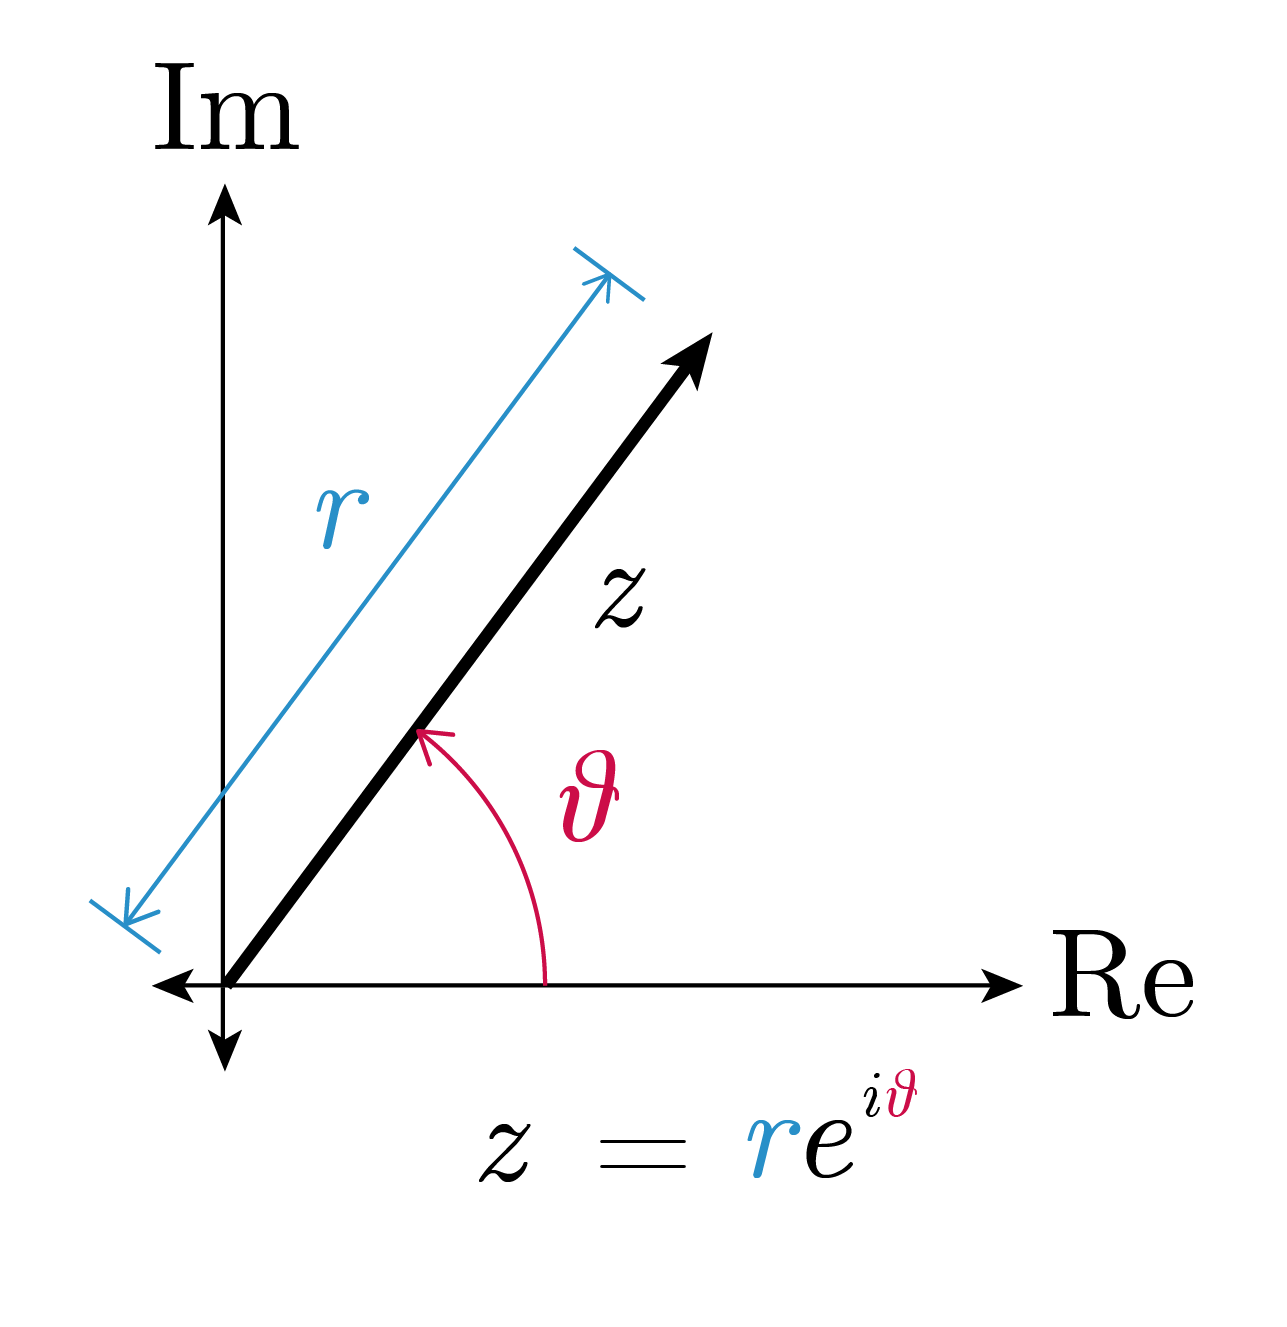
\includegraphics[width=3in]{complex_number_diagram-02}
\end{figure}
We can also express complex numbers with polar coordinates;
see Figure~\ref{fig:polar}.  If we define $r=\abs{z}$
and $\theta$ as the angle from the positive real axis to the Euclidean vector
representation of $z$, then 
\begin{align}
x &= r \cos{\theta} \\
y &= r \sin{\theta}
\end{align}
Using Euler's formula, which I will simply state here as 
\[
e^{i \theta} = \cos{\theta} + i \sin{\theta},
\]
we can also express the complex number $z$ as $z=r e^{i \theta}$.
\subsection{Complex Differentiation}
\subsubsection{Cauchy-Riemann Equations}
\subsection{Contour Integration}
\subsection{Residue Calculus}
\section{Harmonic Analysis}
\label{HarmonicAnalysis}
\subsection{Fourier Series}
\subsection{The Fourier Transform}
\subsection{The Laplace Transform}
\end{document}
